%\newpage
\subsection{Подготовка производства}
\label{bp:Prepare}
%

Единая форма для сбора входящей информации (опросный лист) отсутствует.
Заказчик присылает требования на изготовления продукции в произвольной форме.

Обработка запроса может производиться на основании образец продукции, предоставленного заказчиком. Полученный от заказчика образец изделия из гофрокартона передается дизайнеру, который производит измерение размеров. Дизайнер производит расчет размеров требуемого изделия из гофрокартона в случае, если заказчик в качестве образца передал упаковываемый товар.

От менеджера дизайнерам поступает заявка (рис. \ref{pic:f16}), где прописываются требования к изделиям. 

Дизайнер переносит данные вручную в шаблон ТК, разработанный в MS EXCEL. Часть данных просчитывается по формуле. Параметры без формул  рассчитываются вручную. Технологическая карта разрабатывается в виде таблицы в MS EXCEL (рис. \ref{pic:f15}).

При разработке технологической карты для изделия, производимого с использованием штампа, менеджер передает в отдел дизайна макет штампа. 
После обработки макет отправляется главному технологу. Главный технолог чертит принимает решение о количестве мест на штампе и информацию передает в виде карандашного рисунка, сделанного своей рукой.
Главный технолог разрабатывает маршрут изготовления ГП. 
После внесения корректировок в ТК, производимых главным технологом, ТК возвращается дизайнерам. Далее дизайнеры отсылают готовый макетом поставщику штампов, размещают заказ на изготовление.

При разработке дизайна менеджер передает дизайнерам эскиз печати. Этот эскиз обрабатывают и передают поставщику клише для изготовления оснастки. 

После создания технологической карты дизайнер отправляет ее на согласование главному технологу. Только после согласования главным технологом ТК направляют менеджеру отдела продаж для утверждения заказчиком. 
  
При необходимости выкрасов дизайнер совместно с колористом определяют номер оттенка по шкале Pantone. Номер кода цвета отсылают в Москву в компанию <<АГ Флекс>>, откуда приходит формула цвета, по которой смешивают краску и делают выкрасы вручную.

Номер технологической карты присваивают дизайнеры.


Готовые технологические карты хранят на сервере в виде таблиц MS EXCEL. К ним имеют доступ все заинтересованные лица без возможности внесения изменений.

При внесении в уже действующую технологическую карту изменений дизайнеры создают новую ТК, которой присваивается новый номер.


\begin{figure}
\begin{center}
 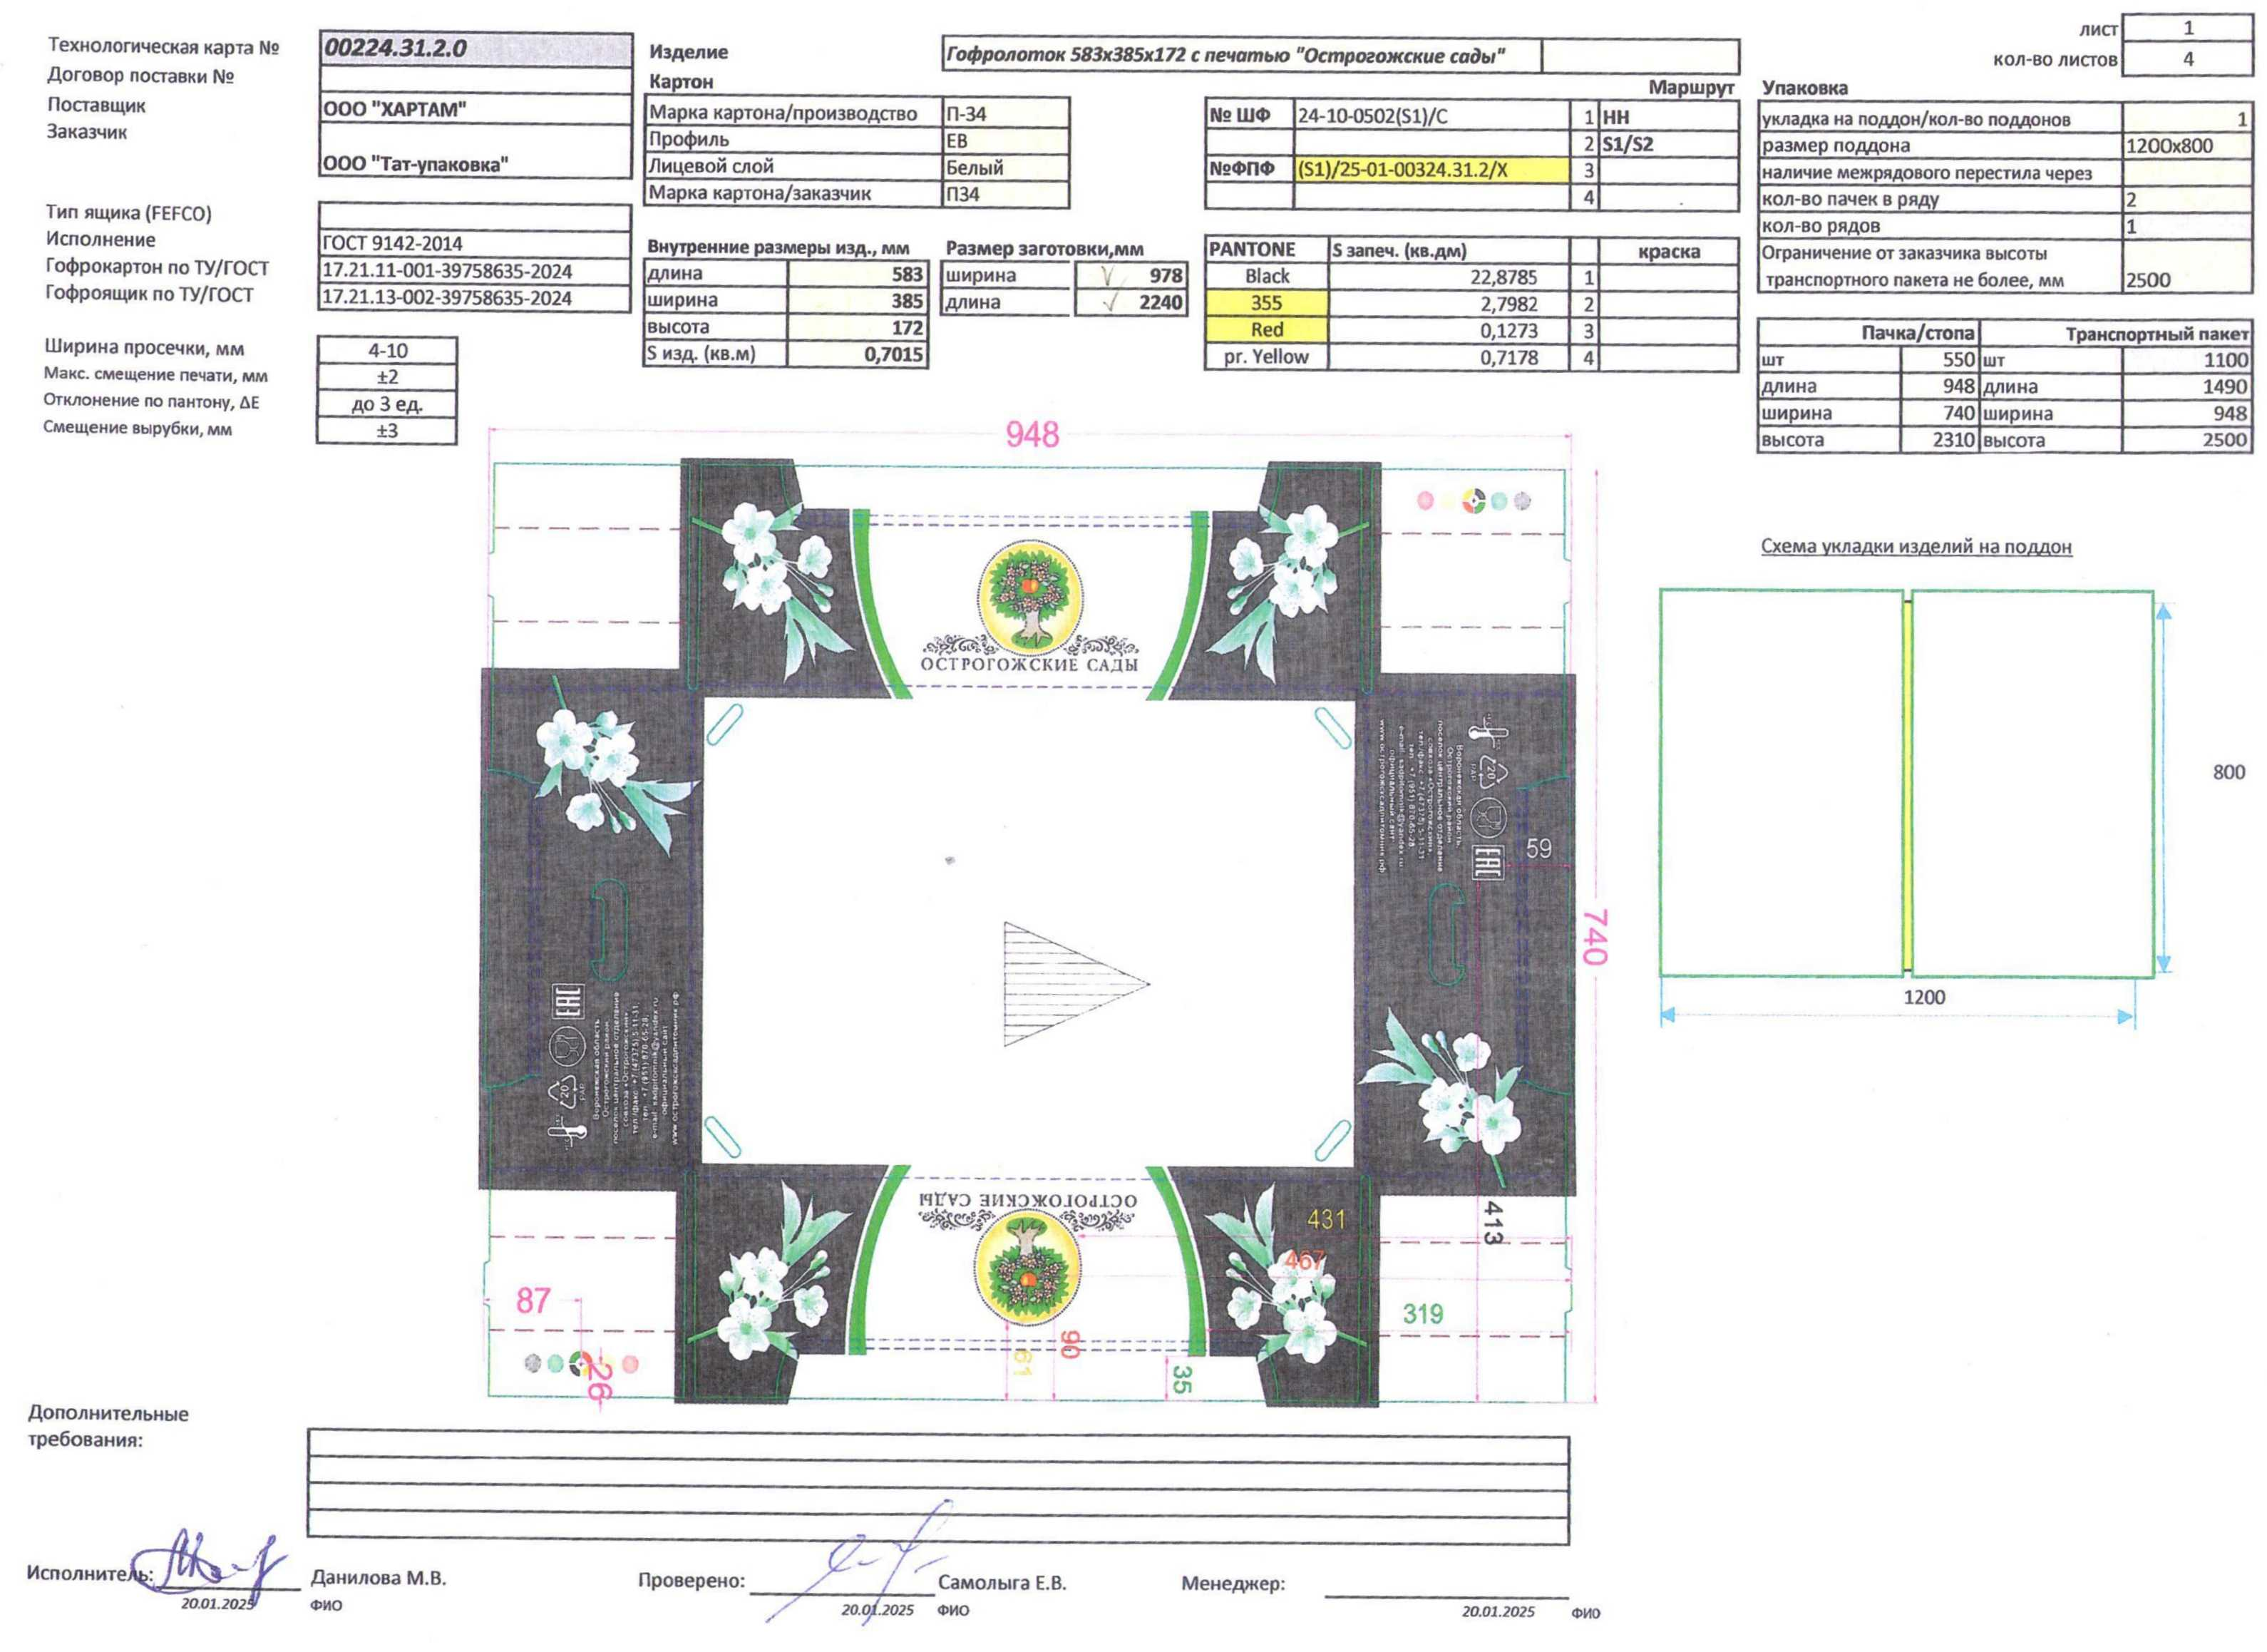
\includegraphics[width=\linewidth, height=0.94\textheight, angle=90, keepaspectratio]{Pics/f15.jpg}
\end{center}
\caption{Разработка ТК}
\label{pic:f15}
\end{figure}

\begin{figure}
\begin{center}
 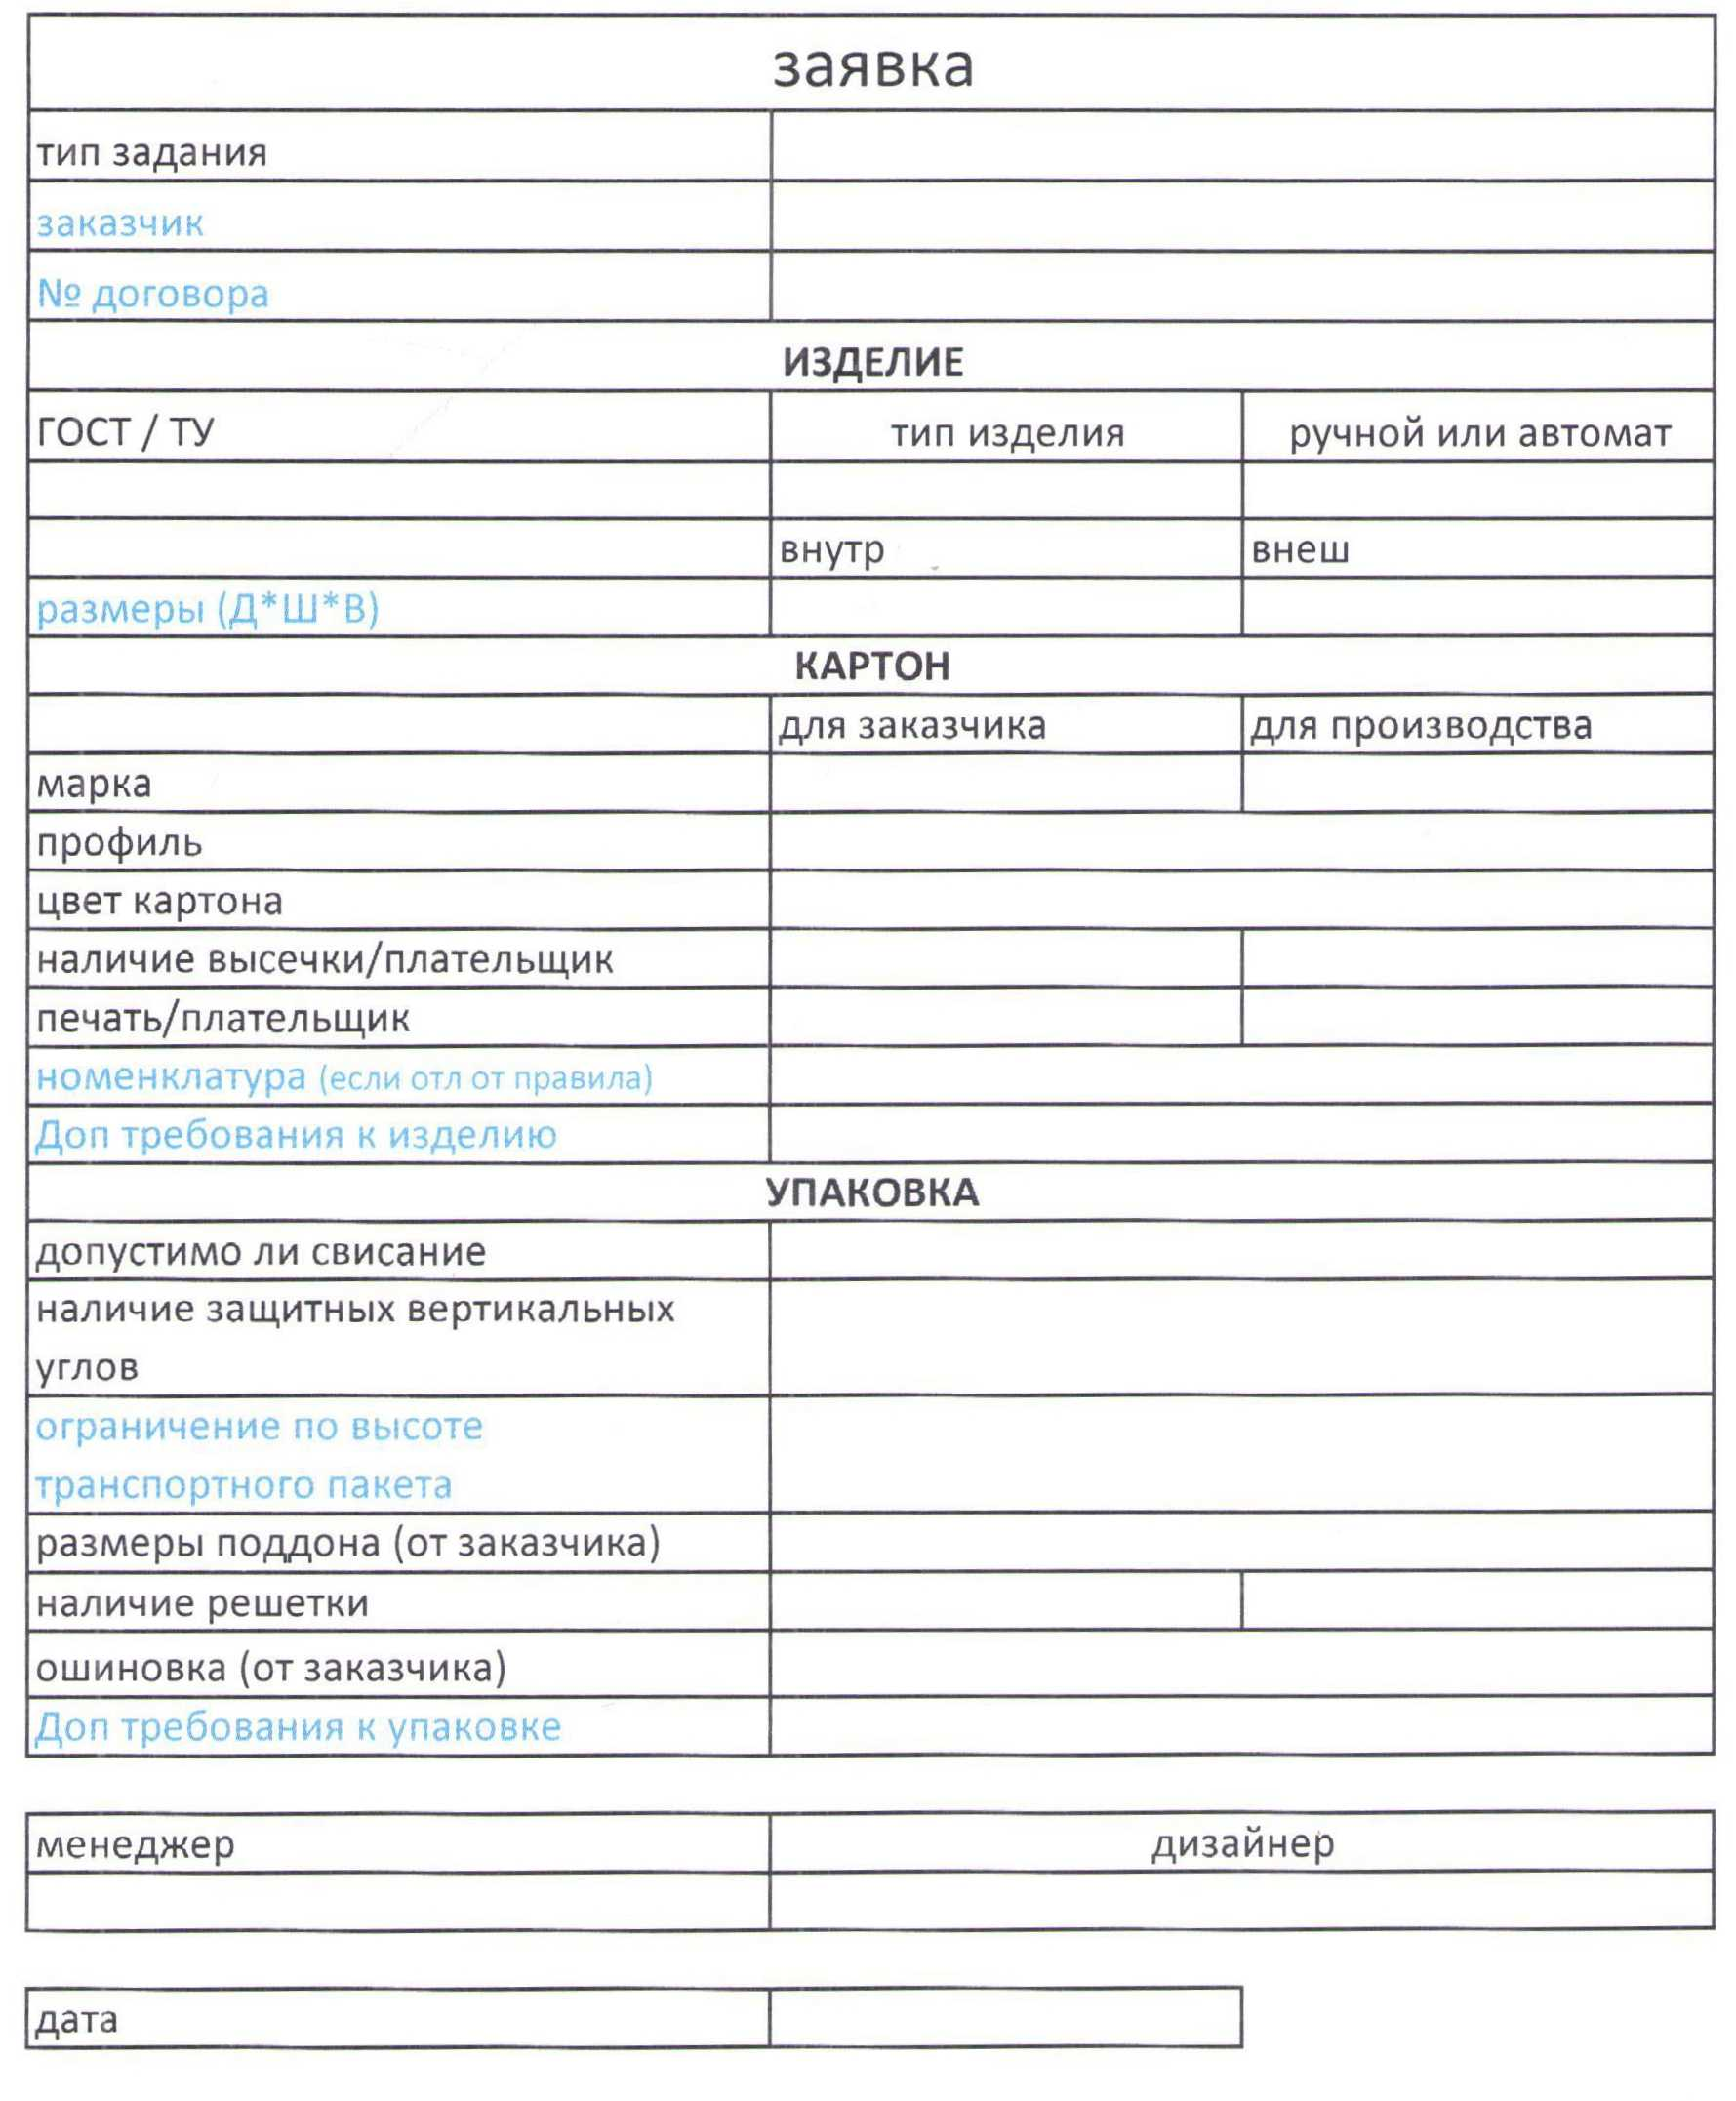
\includegraphics[width=\linewidth, height=0.94\textheight, keepaspectratio]{Pics/f16.jpg}
\end{center}
\caption{Заявке на разработку чертежа и макета}
\label{pic:f16}
\end{figure}
%\end{figure}


\clearpage
\ifx \notincludehead\undefined
\normalsize
\end{document}
\fi